\documentclass[t,usenames,dvipsnames]{beamer}
\usetheme{Copenhagen}
\setbeamertemplate{headline}{} % remove toc from headers
\beamertemplatenavigationsymbolsempty

\usepackage{amsmath, tkz-euclide, tikz, xcolor, pgfplots, array}
\usetkzobj{all}
\pgfplotsset{compat = 1.16}
\usetikzlibrary{arrows.meta, calc, decorations.pathreplacing}
\pgfplotsset{every axis/.append style = {axis lines = middle, axis line style = {<->}}}
\pgfplotsset{every tick label/.append style={font=\scriptsize}}
\everymath{\displaystyle}

\title{Functions and Their Graphs}
\author{}
\date{}

\AtBeginSection[]
{
  \begin{frame}
    \frametitle{Objectives}
    \tableofcontents[currentsection]
  \end{frame}
}

\begin{document}

\begin{frame}
    \maketitle
\end{frame}

\section{Determine if a relation is a function.}

\begin{frame}{Vocab}
    A \alert{relation} is a set of ordered pairs.  \newline\\
    
    The \alert{domain} is the set of all input values (usually $x$).   \newline\\
    
    The \alert{range} is the set of all output values (usually $y$).
\end{frame}

\begin{frame}{Relations and Functions}
    A relation is a \alert{function} if each element in the domain has only 1 corresponding element in the range.  \newline\\
    
    In other words, each $x$-coordinate has only 1 $y$-coordinate.
\end{frame}

\begin{frame}{Example 1}
Which of the following describes $y$ as a function of $x$? For the ones that do, state the domain and range.  \newline\\

(a) \quad $\{(-2,1), \, (1, 3), \, (1, 4), \, (3, -1)\}$ \newline\\  \pause
\[\{(-2,1), \, ({\color{red} 1}, 3), \, ({\color{red} 1}, 4), \, (3, -1)\}\]    \pause

Not a function ($x=1$ has 2 different $y$-coordinates)
\end{frame}

\begin{frame}{Example 1}
(b) \quad   $\{(-2,1), \, (1,3),  \, (2,3), \, (3,-1)\}$    \newline\\  \pause

Since all $x$-coordinates are different, this IS a function.    \newline\\  \pause

Domain: $-2, \, 1, \, 2, \, 3$  \newline\\
Range: $-1, \, 1, \, 3$
\end{frame}

\begin{frame}{Vertical Line Test}
If you are given the equation, you can graph it and use the \alert{Vertical Line Test}: \newline\\ \pause
\begin{enumerate}
    \item<+-> Graph the equation.   \newline\\
    \item<+-> Draw vertical lines through the graph.    \newline\\
    \item<+-> If each vertical line hits the graph only once (or not at all), it is a function.
\end{enumerate}
\end{frame}

\begin{frame}{Example 2}
Determine if each defines $y$ as a function of $x$. \newline\\
(a) \quad   $x^2 + y = 4$   \newline\\  \pause
\begin{minipage}{0.5\textwidth}
\begin{tikzpicture}[scale=0.85]
\begin{axis}[
    xmin = -4.25, xmax = 4.25,
    ymin = -5.25, ymax = 5.25,
]
\addplot[<->, blue, very thick, domain=-2.75:2.75] {4-x^2};
\end{axis}
\end{tikzpicture}
\end{minipage}
\hspace{0.25cm}
\begin{minipage}{0.4\textwidth}
\onslide<3->{
Passes Vertical Line Test   \newline\\
Is a function.}
\end{minipage}
\end{frame}

\begin{frame}{Example 2}
(b) \quad $x^2 + y^2 = 4$   \newline\\  \pause
\begin{minipage}{0.5\textwidth}
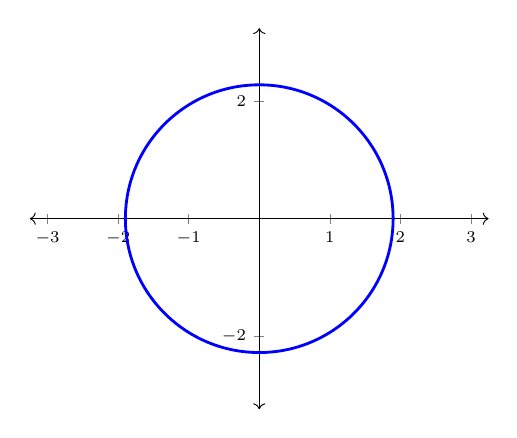
\begin{tikzpicture}[scale=0.85]
\begin{axis}[
    xmin = -3.25, xmax = 3.25,
    ymin = -3.25, ymax = 3.25,
]    
\draw [blue, very thick] (axis cs: 0,0) circle (2cm);
\end{axis}
\end{tikzpicture}
\end{minipage}
\hspace{0.45cm}
\begin{minipage}{0.4\textwidth}
\onslide<3->{
Fails Vertical Line Test    \newline\\
Not a function}
\end{minipage}
\end{frame}

\begin{frame}{Example 2}
(c) \newline\\  
\begin{minipage}{0.5\textwidth}
\begin{tikzpicture}[scale=0.8]
\begin{axis}[
    xmin = -2, xmax = 2,
    ymin = -1
]
    \addplot [blue, domain = -1.5:1.75,samples=300, <->, very thick]
      {x^2 - 0.5};
    \plot [fill = black] (1,1.5) circle (3pt);
\end{axis}
\end{tikzpicture}
\end{minipage} 
\hspace{0.45cm}
\begin{minipage}{0.4\textwidth}
\onslide<2->{
Fails Vertical Line Test    \newline\\
Not a Function}
\end{minipage}
\end{frame}

\begin{frame}{Example 2}
(d) \newline\\  
\begin{minipage}{0.5\textwidth}
\begin{tikzpicture}[scale=0.8]
\begin{axis}[
    xmin = -2, xmax = 2,
    ymin = -1
]
    \addplot [blue, domain = -1.5:1.75,samples=300, <->, very thick]
      {x^2 - 0.5};
    \plot [fill = black] (1,1.5) circle (3pt);
    \plot [color=blue, fill = white] (1,0.5) circle (3pt);
\end{axis}
\end{tikzpicture}
\end{minipage} 
\hspace{0.45cm}
\begin{minipage}{0.4\textwidth}
\onslide<2->{
Passes Vertical Line Test    \newline\\
Is a Function}
\end{minipage}
\end{frame}

\section{Evaluate functions using function notation.}

\begin{frame}{Function Notation}
We typically use function notation such as $f(x)$ or $g(x)$ when writing functions rather than $y$. \newline\\

To evaluate a function, substitute the value in parentheses into the function.
\end{frame}


\begin{frame}{Example 3}
For $f(x) = -x^2 + 3x + 4$, evaluate each.  \newline\\
(a) \quad $f(-1)$
\begin{align*}
    \onslide<2->{f(-1) &= -(-1)^2 + 3(-1) + 4} \\
    \onslide<3->{&= -1 - 3 + 4} \\
    \onslide<4->{&= 0}
\end{align*}
\end{frame}

\begin{frame}{Example 3}
(b) \quad $f(0)$
\begin{align*}
    \onslide<2->{f(0) &= -(0)^2 + 3(0) + 4} \\
    \onslide<3->{&= 0 + 0 + 4} \\
    \onslide<4->{&= 4}
\end{align*}
\end{frame}

\begin{frame}{Example 3}
(c) \quad   $f(2)$
\begin{align*}
    \onslide<2->{f(2) &= -(2)^2 + 3(2) + 4} \\
    \onslide<3->{&= -4 + 6 + 4} \\
    \onslide<4->{&= 6}
\end{align*}
\end{frame}

\section{Find the domain of a function.}

\begin{frame}{Domains}
As we progress in the course, we will look at various functions; many having restrictions on what input values they will allow.    \newline\\  \pause

Restricted Domains: \newline\\ \pause
\begin{itemize}
    \item<+-> Taking an even ($\sqrt{}, \, \sqrt[4]{}, \, \sqrt[6]{}$, etc.) of a \alert{negative number}.  \newline\\
    \item<+-> Dividing by 0.
\end{itemize}
\end{frame}

\begin{frame}{Example 4}
Find the domain of each.    \newline\\
(a) \quad $g(x) = \sqrt{4-3x}$
\begin{align*}
    \onslide<2->{4 - 3x & \geq 0} \\[5pt]
    \onslide<3->{-3x & \geq -4} \\[5pt]
    \onslide<4->{x & \leq \frac{4}{3}}
\end{align*}

\onslide<5->{\[  \left(-\infty, \frac{4}{3}\right]   \]}
\end{frame}


\begin{frame}{Example 4}
(b) \quad $h(x) = \sqrt[5]{4-3x}$
\onslide<2->{\[(-\infty, \infty)\]}
\end{frame}


\begin{frame}{Example 4}
(c) \quad   $f(x) = \dfrac{2}{1-\dfrac{4x}{x-3}}$
\begin{align*}
    \onslide<2->{x - 3 & \neq 0}    \\
    \onslide<3->{x & \neq 3}
\end{align*}
\end{frame}


\begin{frame}{Example 4}
(c) \quad   $f(x) = \dfrac{2}{1-\dfrac{4x}{x-3}}$\onslide<2->{$\left(\frac{x-3}{x-3}\right)$}
\begin{align*}
    \onslide<3->{&= \dfrac{2(x-3)}{x-3-4x}} \\[6pt]
    \onslide<4->{x - 3 - 4x & \neq 0}   \\
    \onslide<5->{-3x-3 &\neq 0} \\
    \onslide<6->{x &\neq -1}
\end{align*}
\end{frame}

\begin{frame}{Example 4}
(c) 
\[ x \neq -1, 3 \]  \pause
\begin{center}
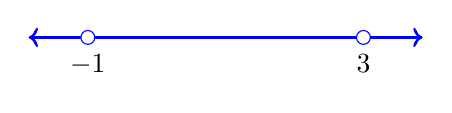
\begin{tikzpicture}
\draw[<->] (-2.5,0) -- (2.5,0);
\draw (-1.75,0.1) -- (-1.75,-0.1) node [below] {$-1$};
\draw (1.75,0.1) -- (1.75,-0.1) node [below] {$3$};
\draw [<->, thick, blue] (-2.5,0) -- (2.5,0);
\draw [color=blue, fill=white] (-1.75,0) circle (2.5pt);
\draw [color=blue, fill=white] (1.75,0) circle (2.5pt);
\end{tikzpicture}
\pause
\end{center}
\[(-\infty, -1) \cup (-1, 3) \cup (3, \infty)\]
\end{frame}

\begin{frame}{Example 4}
(d) \quad $F(x) = \dfrac{\sqrt[4]{2x+1}}{x^2-1}$
\begin{align*}
    \onslide<2->{2x+1 &\geq 0} \\[8pt]
    \onslide<3->{2x &\geq -1} \\[8pt]
    \onslide<4->{x &\geq -\frac{1}{2}} \\
\end{align*}
\end{frame}


\begin{frame}{Example 4}
(d) \quad $F(x) = \dfrac{\sqrt[4]{2x+1}}{x^2-1}$
\begin{align*}
    \onslide<2->{x^2 -1 &\neq 0} \\[8pt]
    \onslide<3->{(x+1)(x-1) &\neq 0} \\[8pt]
    \onslide<4->{x &\neq -1, 1} \\
\end{align*}
\end{frame}


\begin{frame}{Example 4}
\[x \geq -\frac{1}{2}, \quad x \neq -1, 1\] \pause
\begin{center}
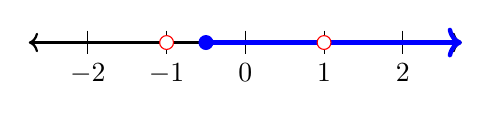
\begin{tikzpicture}
    \draw[<->, thick] (-2.75,0) -- (2.75,0);
    \foreach \x in {-2,-1,0,1,2}
    \draw (\x, 0.15) -- (\x, -0.15) node [below] {$\x$};
    \onslide<3->{\draw [->, ultra thick, blue] (-0.5,0) -- (2.75,0);}
    \onslide<3->{\draw [color=blue, fill=blue] (-0.5,0) circle (2.5pt);}
    \onslide<4->{\draw[color=red, fill=white] (-1,0) circle (2.5pt);}
    \onslide<4->{\draw [color=red, fill=white] (1,0) circle (2.5pt);}
\end{tikzpicture}
\end{center}    
\onslide<5->{\[ \left[-\frac{1}{2}, 1\right) \cup (1, \infty) \]}
\end{frame}

\begin{frame}{Example 4}
(e) \quad $r(t) = \dfrac{4}{6-\sqrt{t+3}}$
\begin{align*}
    \onslide<2->{t +3 & \geq 0} \\[5pt]
    \onslide<3->{t & \geq -3} 
\end{align*}
\end{frame}

\begin{frame}{Example 4}
(e) \quad $r(t) = \dfrac{4}{6-\sqrt{t+3}}$
\begin{align*}
    \onslide<2->{6-\sqrt{t+3} &\neq 0} \\[5pt]
    \onslide<3->{6 &\neq \sqrt{t+3}} \\[5pt]
    \onslide<4->{6^2 &\neq (\sqrt{t+3})^2} \\[5pt]
    \onslide<5->{36 &\neq t+3} \\[5pt]
    \onslide<6->{t &\neq 33}
\end{align*}
\end{frame}

\begin{frame}{Example 4}
    \[ t \geq -3, \quad t \neq 33 \]    \pause
    \begin{center}
        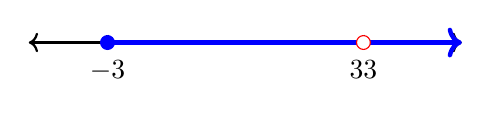
\begin{tikzpicture}
        \draw[<->, thick] (-2.5,0) -- (3,0);
        \draw[thick] (-1.5,0.1) -- (-1.5,-0.1) node [below] {$-3$};
        \draw[thick] (1.75,0.1) -- (1.75,-0.1) node [below] {$33$};
        \onslide<3->{\draw[ultra thick, ->, blue] (-1.5,0) -- (3,0);}
        \onslide<3->{\draw[color=blue, fill=blue] (-1.5,0) circle (2.5pt);}
        \onslide<4->{\draw[color=red, fill=white] (1.75,0) circle (2.5pt);}
        \end{tikzpicture}
    \end{center}
    \onslide<5->{\[[-3, 33) \cup (33, \infty)\]}
\end{frame}

\begin{frame}{Example 4}
(f) \quad $I(x) = \dfrac{3x^2}{x}$  \pause
\begin{align*}
    \onslide<2->{x &\neq 0}
\end{align*}
\pause
\begin{center}
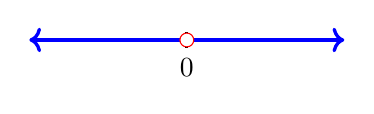
\begin{tikzpicture}
\draw[<->, very thick, blue] (-2,0) -- (2,0);
\draw[very thick] (0,0.1) -- (0,-0.1) node [below] {0};
\draw[color=red, fill=white] (0,0) circle (2.5pt);
\end{tikzpicture}
\end{center}
\pause
\[(-\infty, 0) \cup (0, \infty)\]
\end{frame}

\section{Find the intercepts of a function}

\begin{frame}{Intercepts}
The \alert{$x$-intercept} of a function is where it crosses the $x$-axis (i.e. the $y$-coordinate is 0).    \newline\\

The \alert{$y$-intercept} of a function is where it crosses the $y$-axis (i.e. the $x$-coordinate is 0).
\end{frame}

\begin{frame}{Example 5}
Find the intercepts of $f(x) = x^2 + 4x + 3$.   \newline\\  \pause
\vspace{11pt}
\begin{minipage}{0.5\textwidth}
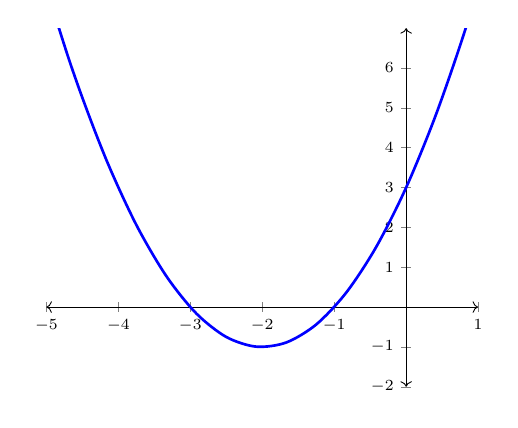
\begin{tikzpicture}[scale=0.8]
\begin{axis}[
    xmin = -5, xmax = 1,
    ymin = -2, ymax = 7,
    ytick = {-2,-1,0,1,2,3,4,5,6}
]    
\addplot[blue, <->, smooth, very thick] {x^2 + 4*x + 3};
\end{axis}
\end{tikzpicture}   \pause
\end{minipage}
\hspace{0.75cm}
\begin{minipage}{0.3\textwidth}
$x$-intercepts: \newline\\  \pause
$(-3,0)$ and $(-1,0)$ \newline\\    \pause
$y$-intercept: $(0,3)$
\end{minipage}
\end{frame}

\end{document}
